\documentclass[10pt,conference]{IEEEtran}
\usepackage[T1]{fontenc}
\usepackage{newtxtext,newtxmath,microtype,graphicx,booktabs,tabularx,array,amsmath,url,balance,float,placeins}
\usepackage[hidelinks]{hyperref}
\usepackage{tikz,xcolor}
\definecolor{deepblue}{HTML}{24578B}
\definecolor{paleBlue}{HTML}{E7F0FA}
\definecolor{paleTeal}{HTML}{E4F5F0}
\definecolor{paleAmber}{HTML}{FFF2D8}
\definecolor{paleGray}{HTML}{F2F4F7}
\usetikzlibrary{arrows.meta,positioning,fit}
\setlength{\tabcolsep}{3pt}
\renewcommand{\arraystretch}{1.10}
\title{From Co-occurring Ambiguities to Action-Ready Robot Tasks: A Study of Structured, Context-Grounded Interpretation}
\author{\IEEEauthorblockN{Mohammed Bangie \hspace{0.5em} (Student No. 2610990)}\IEEEauthorblockA{School of Computer Science and Applied Mathematics\\University of the Witwatersrand, Johannesburg, South Africa\\Supervisors: Steven James and Benjamin Rosman}}
\newcommand{\pending}[1]{\noindent\textit{[Pending: #1]}\par}
\begin{document}
\maketitle\thispagestyle{plain}\pagestyle{plain}
\begin{abstract}
A single instruction to a robot may contain several ambiguities at once: an indirect request, an unclear object reference, an imprecise time, or a missing destination. These ambiguities need not prevent action if the surrounding scene and conversation provide enough information to resolve them. The challenge is therefore not simply to detect ambiguous language, but to recover the intended task without inventing details or asking unnecessary questions. This paper studies a text-to-text approach that converts human instructions, scene descriptions, dialogue history, and robot capability descriptions into action-ready task specifications. The proposed approach uses Qwen3 to identify the intended goal, construct a structured task with evidence for its arguments, and request clarification only when an essential detail remains unresolved. We define controlled comparisons against direct generation and an optional repeated-Qwen3 review, together with tests of context removal, intermediate structure, and dependency checking. A co-occurring ambiguity dataset of 99 instructions supports the evaluation design. Its task interpretations were adjudicated by the author after review by GLM-5.2, Grok 4.5, and GPT-5.6 Sol. The study examines task interpretation, grounding, and clarification efficiency without assuming that additional reasoning calls necessarily help.
\end{abstract}
\begin{IEEEkeywords}
Human--robot interaction, language grounding, ambiguity resolution, clarification, task specification, large language models.
\end{IEEEkeywords}
\section{Introduction}
People rarely describe everyday tasks as complete lists of robot actions. A person might say, ``Put the other cup beside the plate on the left, then move it over there.'' The robot must determine which cup and plate are meant, what ``left'' refers to, whether ``it'' denotes the cup or plate, and where the final destination is. Some answers may be present in the scene or earlier conversation; others may require a question. The useful outcome is not a fluent paraphrase but a task description with the right actions, objects, and constraints.

We call a command \emph{co-occurringly ambiguous} when it contains at least two potentially uncertain aspects, such as its intended action, object, location, time, or scope. Co-occurrence does not necessarily mean that the ambiguities depend on each other. For example, identifying a tray may also identify its assigned recipient, whereas choosing a time and choosing a shelf may be independent decisions. The number of ambiguous expressions alone therefore cannot tell us whether the robot should ask for help.

Prior work has studied indirect requests in task-oriented dialogue \cite{mannekote}, classification and clarification of robot commands \cite{clara}, clarification requests during collaborative tasks \cite{codraw}, and mapping vague commands to structured control calls \cite{clarifyvc}. These studies provide important methods, but they do not by themselves establish which combination is necessary to turn instructions with several ambiguity types into fully grounded task specifications. Work on integrating language models into robotic architectures also cautions against evaluating language interpretation only as an isolated fluent output \cite{sarathy}.

Our scope is deliberately limited to \emph{text-to-text interpretation}. The input may describe a physical environment and the robot's available actions, but this study does not perform motion planning or test physical execution. We define an \emph{action-ready task} as a structured description whose required actions, arguments, and constraints are determined from the supplied information or an explicit user clarification. Action readiness does not certify that a real robot can safely execute the task.

This paper sets out three contributions to be evaluated: (i) a goal-first, evidence-grounded task representation that distinguishes resolved details from unresolved ones; (ii) a controlled study of whether this structure and its contextual checks improve over direct Qwen3 generation; and (iii) an analysis of whether a second Qwen3 interpretation and optional adjudication justify their additional cost. These are research aims, not claims of demonstrated improvements.

\section{Background and Related Work}
\subsection{Indirect meaning and task interpretation}
A request can communicate an intended action without naming that action directly. Searle distinguishes the literal form of an utterance from an indirect act performed through it \cite{searle1975}, while Grice explains how conversational context supports inferences beyond the words explicitly spoken \cite{grice1975}. These accounts motivate interpreting communicative intent, but do not supply an algorithm for generating action-ready robot tasks. Mannekote \emph{et al.} study the synthetic generation of indirect requests to make task-oriented dialogue data more natural \cite{mannekote}. Zhang \emph{et al.} examine indirect speech in physical human--robot collaboration, where the literal wording and intended collaborative response may differ \cite{tool}. These works establish why interpreting only the surface wording is inadequate. They do not, however, provide a general test of multiple interacting ambiguities within one task specification.

\subsection{Ambiguity and contextual grounding}
AmbiK provides ambiguous task instructions situated in kitchen environments, illustrating how the same instruction can require additional knowledge or clarification \cite{ambik}. VAGUE investigates how visual context can clarify ambiguous expressions \cite{vague}. Context can make one interpretation more plausible than another, but a plausible interpretation still needs evidence.

A useful distinction is between \emph{co-occurrence} and \emph{dependence}. Two ambiguous fields co-occur when both appear in an instruction; they depend on one another when choosing a value for one constrains the possible value of the other. For example, selecting a labelled medicine tray may determine its recipient. In contrast, the tray and an unrelated delivery deadline may each be resolved independently. This distinction affects how ambiguity is evaluated, even when both instructions contain the same number of ambiguity labels.

\subsection{Clarification in human--robot interaction}
CLARA classifies commands using the current situation and supports clarification of ambiguous instructions \cite{clara}. Madureira and Schlangen analyse clarification requests in collaborative CoDraw dialogues, showing that clarification can concern specific missing or uncertain task information \cite{codraw}. An important distinction is that uncertainty about a model prediction does not necessarily mean a required task detail is missing. For the present text-to-text problem, clarification must ultimately be judged by whether it resolves an execution-critical field.

\subsection{Structured task generation and robot capabilities}
ClarifyVC studies the translation of ambiguous vehicle-control commands into structured, schema-aligned calls and uses ambiguity-oriented data augmentation \cite{clarifyvc}. This makes it a close methodological reference, although vehicle functions are more constrained than many general robot tasks. The Qwen3 technical report describes the language-model family used in this study, including its thinking and non-thinking modes \cite{qwen}. Because Qwen3 already supports internal reasoning, a multi-stage procedure must be evaluated against a strong direct-generation baseline with thinking enabled; additional prompts alone do not establish a new reasoning capability.

\subsection{Research gap}
The literature provides complementary accounts of indirect meaning, grounding, clarification, and structured outputs. The open question addressed here is narrower and testable: for commands containing several ambiguities, does explicitly representing a task's goal, grounded arguments, and unresolved details improve the correctness of the final task compared with direct generation? A related question is whether repeated reasoning with the same model adds value beyond the structured approach. These questions require reference task specifications, not only labels such as ``execute'' and ``clarify.''

\section{Research Questions and Hypotheses}
\textbf{RQ1 (structured interpretation):} Does an explicit, evidence-grounded task representation with action-readiness validation improve complete-task correctness over direct generation with the same Qwen3 checkpoint, input context, and comparable inference budgets?

\emph{H1:} Structured interpretation will increase the proportion of fully correct task specifications and reduce unsupported argument choices relative to direct generation.

\textbf{RQ2 (context and ambiguity dependence):} How do scene descriptions, dialogue history, and explicit checks between task arguments affect correct interpretation, particularly when ambiguities depend on each other?

\emph{H2:} Removing relevant context will reduce grounding accuracy; checking dependencies will be most useful for examples with linked arguments, rather than all multi-ambiguity examples equally.

\textbf{RQ3 (repeated reasoning):} Does an additional independent Qwen3 interpretation, with optional Qwen3 adjudication, improve correctness enough to justify extra inference cost?

\emph{H3:} Review may correct some initial interpretations, but its net benefit will be smaller when compared with a structured system given a comparable inference budget. This hypothesis may be rejected if review adds no measurable value.

\section{Methodology}
\subsection{Task and output definition}
The system receives a human instruction $u$, a scene description $s$, previous dialogue $d$, and a list of available robot actions and their required arguments $c$. Its input is
\begin{equation}
 x=(u,s,d,c),\qquad f(x)\in\{T,q\},
 \label{eq:task}
\end{equation}
where $T$ is a structured task and $q$ is a clarification question. The task $T$ contains the intended goal, ordered actions, their arguments, constraints, and evidence for the chosen values. Missing values remain explicitly unresolved rather than being guessed. For the set $R(T)$ of required arguments, we define
\begin{equation}
 \operatorname{Ready}(T)=
 \left[\bigwedge_{a\in R(T)}\operatorname{Grounded}(a,x)\right]
 \land\operatorname{Consistent}(T,c).
 \label{eq:ready}
\end{equation}
Here, $\operatorname{Grounded}(a,x)$ means that the value of argument $a$ is supported by the instruction, scene, dialogue, or an explicit clarification; $\operatorname{Consistent}(T,c)$ means that the task uses valid action arguments and contains no conflicting constraints. These are criteria for a text specification, not a claim of safe or successful physical execution.

\subsection{Co-occurring ambiguity dataset}
We use one \emph{co-occurring ambiguity dataset} containing 99 instructions. Each record provides a human utterance, scene description, available dialogue history, robot capabilities, ambiguity-type labels, and an execute-or-clarify reference decision. The dataset contains 76 execute and 23 clarify decisions in its recorded routing labels. It also contains intended goals, ordered actions, grounded objects and parameters, supporting contextual evidence, unresolved critical fields, dependencies between fields, and clarification questions with conditional answers. Together, these annotations support evaluation of complete task interpretation, grounding correctness, and clarification necessity rather than routing alone.

The dataset was reviewed using GLM-5.2 \cite{glm52} and Grok 4.5 \cite{grok45}, with GPT-5.6 Sol \cite{gpt56sol} used for model-assisted reconciliation. The author, Mohammed Bangie, then personally adjudicated the reference interpretations. Model-assisted review and the author's human adjudication are distinct stages; model agreement alone was not treated as proof of correctness. Conditional clarification answers represent annotated scenarios rather than observed conversations. The 99 cases are held out for evaluation, not used for prompt tuning or model selection.

\subsection{Proposed interpretation pipeline}
Fig.~\ref{fig:pipeline} summarizes the interpretation process. In the mandatory path, Qwen3 first identifies the intended goal and possible ordered subtasks without treating every plausible inference as a fact. Second, Qwen3 constructs a task representation, attaching scene or dialogue evidence to object choices, times, destinations, and constraints. Where one choice determines another, the representation records that relationship. The optional independent Qwen3 review branches from the grounded interpretation and, when enabled, reconciles disagreements before validation. Third, validation checks schema completeness, permitted action names, argument references, and internal consistency. Mechanical checks are deterministic where possible; semantic support remains an evaluated model judgment. When a critical field is unresolved, the system asks a targeted question; the answer returns to task grounding before the revised task is validated again. Clarification is capped at five turns in the planned protocol; reaching the cap without a complete task counts as unresolved.

\begin{figure}[!b]
\centering
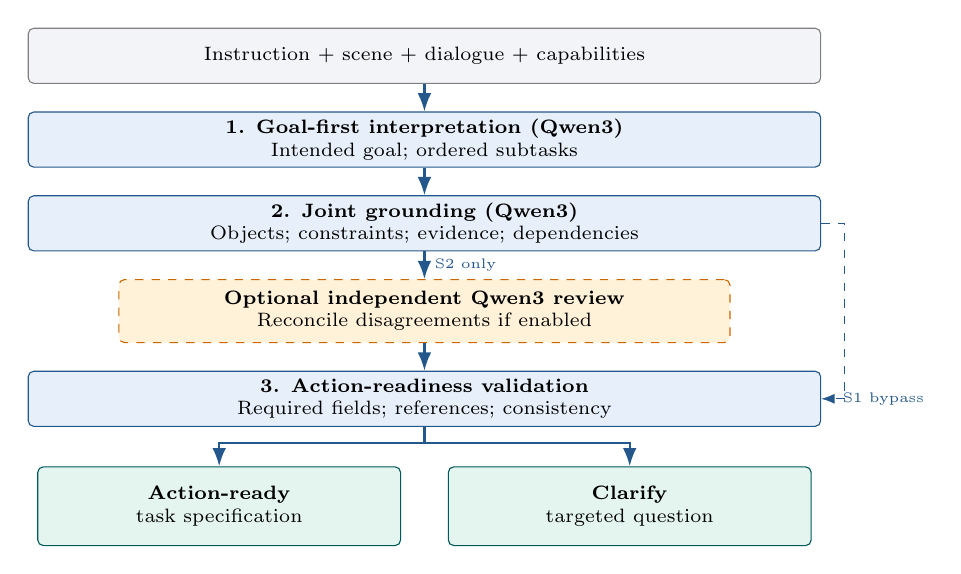
\begin{tikzpicture}[font=\scriptsize,>=Latex,node distance=3.5mm,
 core/.style={draw=deepblue,fill=paleBlue,rounded corners=2pt,minimum width=.83\columnwidth,minimum height=7mm,inner sep=2pt,align=center},
 input/.style={core,fill=paleGray,draw=gray},
 opt/.style={draw=orange!80!black,fill=paleAmber,dashed,rounded corners=2pt,minimum width=.64\columnwidth,minimum height=8mm,align=center,inner sep=2pt},
 resultbox/.style={draw=teal!70!black,fill=paleTeal,rounded corners=2pt,minimum width=.38\columnwidth,minimum height=10mm,align=center,inner sep=2pt}]
\node[input] (i) {Instruction + scene + dialogue + capabilities};
\node[core,below=of i] (g) {\textbf{1. Goal-first interpretation (Qwen3)}\\Intended goal; ordered subtasks};
\node[core,below=of g] (t) {\textbf{2. Joint grounding (Qwen3)}\\Objects; constraints; evidence; dependencies};
\node[opt,below=of t] (r) {\textbf{Optional independent Qwen3 review}\\Reconcile disagreements if enabled};
\node[core,below=of r] (v) {\textbf{3. Action-readiness validation}\\Required fields; references; consistency};
\node[resultbox,below=5mm of v,xshift=-.215\columnwidth] (ok) {\textbf{Action-ready}\\task specification};
\node[resultbox,below=5mm of v,xshift=.215\columnwidth] (ask) {\textbf{Clarify}\\targeted question};
\draw[->,thick,deepblue] (i)--(g);
\draw[->,thick,deepblue] (g)--(t);
\draw[->,thick,deepblue] (t)--node[right,font=\tiny]{S2 only}(r);
\draw[->,thick,deepblue] (r)--(v);
\draw[->,thick,deepblue] (v.south)--++(0,-2mm)-|(ok.north);
\draw[->,thick,deepblue] (v.south)--++(0,-2mm)-|(ask.north);
\draw[->,dashed,deepblue] (t.east) -- ++(3mm,0) |- node[pos=.75,right,font=\tiny]{S1 bypass}(v.east);
\end{tikzpicture}
\caption{Proposed interpretation pipeline. S1 bypasses the optional review; S2 includes it. Clarification answers are incorporated into grounding and revalidated (feedback omitted for legibility).}
\label{fig:pipeline}
\end{figure}

\FloatBarrier
\subsection{Worked example: one choice resolves two fields}
Table~\ref{tab:worked} illustrates the difference between detecting several ambiguities and identifying the particular information needed to complete a task. The example is drawn from case CA-0007 in the co-occurring ambiguity dataset. Its scene identifies two selected medicine trays, assigned respectively to a nurse and a ward clerk. Dialogue establishes that the utterance is a delivery request, and the relevant meal service is at 11:00. Neither fact identifies which tray to deliver. The tray choice is therefore unresolved even though the intended action and time are recoverable.
\begin{table}[!tbp]
\caption{Illustrative grounded interpretation of CA-0007; the user reply is hypothetical, not observed.}
\label{tab:worked}
\centering\footnotesize
\renewcommand{\arraystretch}{1.26}
\begin{tabularx}{\columnwidth}{@{}p{.25\columnwidth}X@{}}
\toprule
\textbf{Element} & \textbf{Interpretation or evidence}\\
\midrule
Utterance & ``Can the selected controlled medicine tray be delivered after a scheduled meal service?''\\
Grounded goal & Deliver a selected controlled medicine tray after the 11:00 meal service.\\
Resolved & Delivery intent; tray type; relevant meal-service time.\\
Missing & Which of the two selected trays is intended?\\
Dependency & Selecting a tray also identifies its assigned recipient.\\
Clarification & ``Which selected controlled medicine tray should I deliver: the nurse's or the ward clerk's?''\\
Conditional output & If the reply is ``the nurse's tray,'' deliver that tray to the nurse after the 11:00 service.\\
\bottomrule
\end{tabularx}
\end{table}
The example shows why a task may contain several ambiguity labels but require only one question. The question resolves the tray choice and, through the assignment recorded in the scene, the recipient. The conditional output is an annotation example, not a measured system prediction. No physical delivery is performed or implied.
\FloatBarrier

\FloatBarrier
\subsection{Main comparisons and controls}
Table~\ref{tab:systems} summarizes the three systems. S0 provides direct generation; S1 is the proposed core system; and S2 tests whether independent repeated reasoning adds value. In S2, the second Qwen3 response is generated without seeing the first, and any adjudication uses the input evidence rather than majority voting. All systems receive the same input information and produce the same output schema. We record inference calls, token usage, and latency, and examine whether S2's extra cost explains any advantage. All stochastic systems are evaluated across repeated runs with fixed, documented random seeds; a single run is not treated as a reliable estimate.

\begin{table}[!tbp]
\caption{Main Qwen3 system comparisons}
\label{tab:systems}
\centering
\footnotesize
\begin{tabularx}{\columnwidth}{@{}p{.12\columnwidth}p{.27\columnwidth}X@{}}
\toprule
\textbf{ID} & \textbf{System} & \textbf{Purpose}\\
\midrule
S0 & Direct Qwen3 & Generate a task or clarification in one pass (baseline).\\
S1 & Structured Qwen3 & Goal-first interpretation, joint grounding, validation, and clarification (core).\\
S2 & S1 + Qwen3 review & Independent second interpretation; optional adjudication of disagreements (extension).\\
\bottomrule
\end{tabularx}
\end{table}

\FloatBarrier
\subsection{Ablations and evaluation}
Within S1, planned ablations remove goal-first interpretation, structured intermediate grounding, scene context, and dependency checks. Dialogue removal is assessed on the subset with dialogue history. For dependency analysis, cases with explicit linked fields are reported separately from cases whose ambiguity labels merely co-occur; this is an exploratory subgroup analysis because the dataset has limited explicitly linked dependency annotations.

The primary measure is \emph{complete task correctness}: whether all required actions, arguments, and constraints match an independently adjudicated reference in meaning. Secondary measures include per-field grounding accuracy, unsupported-argument rate, missing-critical-field rate, execute/clarify decisions, unnecessary clarification, clarification turns, and inference cost per correctly resolved task. Equivalent task descriptions are judged semantically rather than by literal JSON string matching. Each system is evaluated over five prespecified repeated runs, with identical cases and documented decoding settings; case-level paired comparisons and uncertainty intervals account for variation across cases and runs. Runs are repeated for the ablations where computationally feasible, and any reduced repetition is reported explicitly. Confidence intervals are not calculated by treating repeated outputs from the same case as independent examples. Any evaluation using simulated answers will be clearly separated from evaluation with real user replies.

\subsection{Failure analysis and scoring procedure}
Every incorrect prediction will be assigned a primary failure category using the same adjudicated reference: wrong intended goal, wrong entity or argument, missing constraint, unsupported inferred detail, unnecessary clarification, or failure to clarify a critical unknown. Secondary tags may be retained when more than one error occurs, but each case contributes once to the primary error count. Reviewers will examine the input evidence and generated structured task, not only the model's explanation. Table~\ref{tab:failure} reserves space for this breakdown in Results.

To score complete task correctness, an evaluator checks the meaning of the full task, including action order and constraints; schema validity alone is insufficient. For a clarification-required case, the initial question is evaluated separately from any task produced after a supplied answer. Disagreements in semantic scoring are resolved using the documented annotation protocol. Results will be reported with the number of eligible cases for each metric.

\subsection{Reproducibility and experimental controls}
Before the first evaluated run, the implementation will record the exact Qwen3 checkpoint identifiers and revisions, inference framework, precision or quantization, hardware, prompt templates, decoding parameters, seeds, and any context-length or output-length limits. All three systems use the same frozen evaluation records, capability information, output schema, and scoring procedure. Five prespecified runs per system measure variation from stochastic decoding; seed variation is not treated as additional independent test cases. Model-call count, generated tokens, and latency are logged for every command. The smaller-checkpoint comparison uses identical test inputs and the same serving hardware where feasible. Thinking mode is recorded explicitly; thinking-enabled and non-thinking configurations are compared under identical inputs, with reasoning tokens included in latency and token-cost accounting. Thinking mode is a controlled inference condition, not a fourth main system. Reasoning-enabled direct generation is the primary baseline; the structured approach is not compared only against a weaker non-thinking configuration.

The protected cases and their enriched reference answers must not be used to tune prompts or select a model checkpoint. The author-adjudicated dataset and evaluation protocol are versioned and frozen before experiments. Any annotation disagreements are recorded for auditability.

\subsection{Latency and smaller-model evaluation}
A smaller Qwen3 checkpoint is evaluated using the same input and output schema to determine whether the structured pipeline remains practical under a tighter inference budget. The smaller checkpoint is included to assess robustness and efficiency, not to manufacture an artificially weak baseline. Direct and structured systems are compared within each checkpoint; thinking mode and reasoning-token budgets are documented and controlled. The exact checkpoint, quantization, hardware, runtime, decoding settings, warm-up procedure, and batch size are documented before measurement. We measure end-to-end wall-clock latency per command, including all sequential model calls, validation, and clarification-question generation, rather than reporting only the time of an individual call. Where supported by the serving stack, we also report time to first token (TTFT), generated tokens per second, input/output token counts, and peak GPU memory. Median and 95th-percentile latency are calculated from repeated runs; warm-up is excluded consistently. Comparisons use the same hardware and serving conditions. Accuracy, latency, and inference cost are reported together to expose any speed--quality trade-off. A smaller model is not selected merely to lower baseline accuracy: any practical recommendation is based on correctness and efficiency together. Thinking-mode comparisons distinguish improvements from additional reasoning computation.

\FloatBarrier
\section{Results}
\noindent\textit{Reporting layout only. Every chart and table in this section is a placeholder; no experimental results are shown. Replace the blank plotting areas and ``Pending'' cells after evaluation.}

\subsection{Action-ready task correctness and routing}
Table~\ref{tab:mainresults} is reserved for the principal comparison across S0, S1, and S2. Complete task correctness is the primary outcome; routing correctness and unsupported arguments provide complementary evidence about whether the task was interpreted without guessing. Report the number of evaluated commands and the same metric definitions for each system.
\begin{table}[!tbp]
\caption{Main-system performance (all entries pending).}
\label{tab:mainresults}
\centering\small
\renewcommand{\arraystretch}{1.35}
\begin{tabularx}{\columnwidth}{@{}l>{\centering\arraybackslash}X>{\centering\arraybackslash}X>{\centering\arraybackslash}X@{}}
\toprule
\textbf{System} & \textbf{Task correct (\%)} & \textbf{Route correct (\%)} & \textbf{Unsupported (\%)}\\
\midrule
S0 & -- & -- & --\\
S1 & -- & -- & --\\
S2 & -- & -- & --\\
\bottomrule
\end{tabularx}
\end{table}
\noindent\textbf{Results commentary to complete (placeholder).}  In the completed report, state which system achieves the highest complete-task accuracy, whether routing and grounding follow the same pattern, and whether observed differences are supported by paired uncertainty intervals. Distinguish an incorrect task from an unnecessary clarification.

\FloatBarrier
\subsection{Stability across repeated runs}
Figure~\ref{fig:runvariation} will display one point for each of five repeated runs per system. The horizontal axis is complete-task correctness; separate rows identify the systems. Add a mean marker and an interval describing variation across runs. This makes instability visible without a large table of individual seeds.
\begin{figure}[!tbp]
\centering
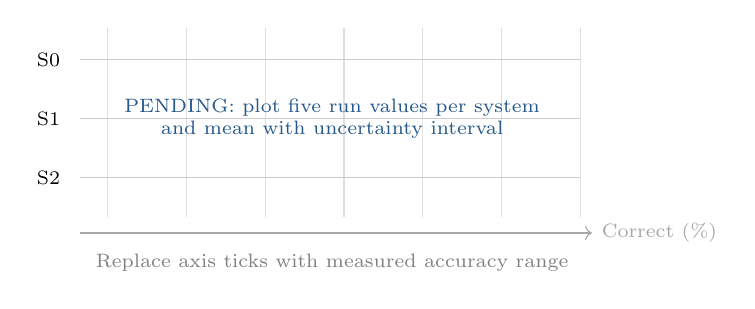
\begin{tikzpicture}[x=1cm,y=1cm,font=\scriptsize]
\draw[->,gray!70] (.65,.35)--(7.15,.35) node[right] {Correct (\%)};
\foreach \x in {1,2,3,4,5,6,7}{\draw[gray!25] (\x,.55)--(\x,2.95);}
\foreach \y/\n in {2.55/S0,1.8/S1,1.05/S2}{\node[anchor=east] at (.52,\y) {\n};\draw[gray!40] (.65,\y)--(7,\y);}
\node[align=center,text=deepblue] at (3.85,1.8) {PENDING: plot five run values per system\\and mean with uncertainty interval};
\node[anchor=north,text=gray] at (3.85,.20) {Replace axis ticks with measured accuracy range};
\end{tikzpicture}
\caption{Temporary plotting template: run-to-run variation in task correctness. No data plotted.}
\label{fig:runvariation}
\end{figure}
\noindent\textbf{Results commentary to complete (placeholder).}  In the completed report, discuss whether rankings remain consistent across seeds, the size of the within-system spread, and whether any apparent improvement is smaller than run-to-run variation. Report case-level paired intervals separately from seed variability.

\noindent\textit{Planned reporting detail.} Each plotted point represents one complete evaluation run on the same frozen set of commands. The visual separates variability from decoding and inference from differences between test cases. The accompanying text will report the five-run mean and standard deviation for each system, while paired case-level intervals will be estimated without treating repeated evaluations of one command as independent observations.

\FloatBarrier
\subsection{Correctness versus latency}
Figure~\ref{fig:tradeoff} will compare primary and smaller Qwen3 checkpoints on the same hardware. Plot end-to-end median latency against complete-task correctness; distinguish systems by marker shape and checkpoint size by colour. Each point represents a system--checkpoint combination, with a horizontal interval for latency variation and a vertical interval for correctness uncertainty when available. The 95th-percentile latency remains an important companion measure in Table~\ref{tab:latency}.
\begin{figure}[!tbp]
\centering
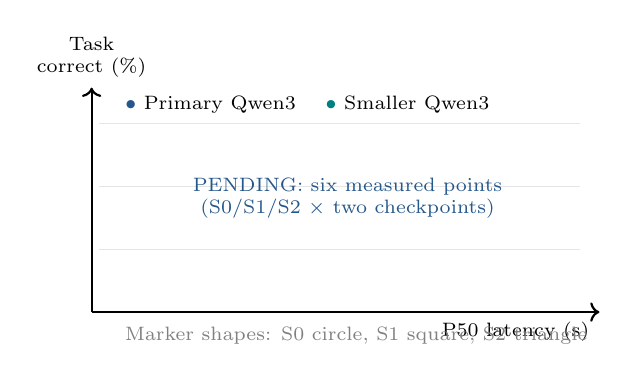
\begin{tikzpicture}[x=1cm,y=1cm,font=\scriptsize]
\draw[->,thick] (.7,.55)--(7.15,.55) node[below left] {P50 latency (s)};
\draw[->,thick] (.7,.55)--(.7,3.4) node[above,align=center] {Task\\correct (\%)};
\draw[gray!20] (.8,1.35)--(6.9,1.35);
\draw[gray!20] (.8,2.15)--(6.9,2.15);
\draw[gray!20] (.8,2.95)--(6.9,2.95);
\node[align=center,text=deepblue] at (3.95,2.0) {PENDING: six measured points\\(S0/S1/S2 $\times$ two checkpoints)};
\node[anchor=west] at (1.0,3.18) {\textcolor{deepblue}{$\bullet$} Primary Qwen3 \quad \textcolor{teal}{$\bullet$} Smaller Qwen3};
\node[anchor=west,text=gray] at (1.0,.25) {Marker shapes: S0 circle, S1 square, S2 triangle};
\end{tikzpicture}
\caption{Temporary plotting template: task correctness versus end-to-end latency. No data plotted.}
\label{fig:tradeoff}
\end{figure}
\begin{table}[!tbp]
\caption{Latency summary (all entries pending).}
\label{tab:latency}
\centering\small
\renewcommand{\arraystretch}{1.32}
\begin{tabularx}{\columnwidth}{@{}lcc>{\centering\arraybackslash}X@{}}
\toprule
\textbf{Checkpoint} & \textbf{System} & \textbf{P50 (s)} & \textbf{P95 (s)}\\
\midrule
Primary & S0/S1/S2 & -- & --\\
Smaller & S0/S1/S2 & -- & --\\
\bottomrule
\end{tabularx}
\end{table}
\noindent\textbf{Results commentary to complete (placeholder).}  In the completed report, identify whether a smaller checkpoint provides an acceptable accuracy--latency trade-off, whether the extra Qwen3 calls in S2 are justified, and whether tail latency changes the practical recommendation. Report the serving configuration and inference cost alongside the final measurements.

\noindent\textit{Planned reporting detail.} The scatter plot will show whether additional inference produces a measurable correctness benefit relative to its time cost. Median latency measures typical response time, whereas the 95th percentile captures slow responses that may be unsuitable for interactive use. Marker shape identifies the pipeline and colour identifies model size; the final figure will include actual units and uncertainty intervals.

\FloatBarrier
\subsection{Component and context ablations}
Table~\ref{tab:ablations} isolates the contribution of intermediate interpretation, grounding, and available context. Differences must be calculated against the corresponding full-S1 result on the same eligible cases, especially for dialogue and linked-dependency subsets.
\begin{table}[!tbp]
\caption{Structured-system ablations (all entries pending).}
\label{tab:ablations}
\centering\small
\renewcommand{\arraystretch}{1.30}
\begin{tabularx}{\columnwidth}{@{}Xcc@{}}
\toprule
\textbf{Configuration} & \textbf{Correct (\%)} & \textbf{$\Delta$ vs. S1 (pp)}\\
\midrule
Full S1 & -- & --\\
Without goal-first interpretation & -- & --\\
Without structured grounding & -- & --\\
Without scene context & -- & --\\
Without dependency checking & -- & --\\
Without dialogue (eligible cases) & -- & --\\
\bottomrule
\end{tabularx}
\end{table}
\noindent\textbf{Results commentary to complete (placeholder).}  In the completed report, describe which removal produces the largest loss, whether context matters more than intermediate structure, and whether dependency checking helps on linked cases rather than only on the full sample. Avoid attributing a causal mechanism to a small numerical difference without supporting case-level evidence.

\noindent\textit{Planned reporting detail.} Every ablation will preserve the evaluation cases and scoring rules of its matched full-system control. Context-removal tests measure sensitivity to available evidence, not performance on an equivalent information task. For the smaller linked-dependency subgroup, results will be reported as exploratory rather than definitive.

\FloatBarrier
\subsection{Error types and qualitative cases}
Table~\ref{tab:failure} will report the dominant causes of incorrect interpretations. This analysis complements overall accuracy by distinguishing errors that might be repaired through more context, better grounding, or targeted clarification. Each category will be illustrated with an anonymized or permitted example, the relevant evidence, and the corrected task interpretation.
\begin{table}[!tbp]
\caption{Failure analysis template (counts and rates pending).}
\label{tab:failure}
\centering\footnotesize
\renewcommand{\arraystretch}{1.32}
\begin{tabularx}{\columnwidth}{@{}Xcc@{}}
\toprule
\textbf{Primary failure type} & \textbf{Count} & \textbf{Rate (\%)}\\
\midrule
Incorrect intended goal & -- & --\\
Wrong entity or argument & -- & --\\
Missing task constraint & -- & --\\
Unsupported inferred detail & -- & --\\
Unnecessary clarification & -- & --\\
Missing required clarification & -- & --\\
\bottomrule
\end{tabularx}
\end{table}
\noindent\textbf{Case interpretation (placeholder).} The completed report will identify which error categories dominate for each system and explain two or three representative cases. It will distinguish failures caused by absent input information from failures to use information already present. Any claim about the value of a component will be supported by its corresponding ablation and case-level evidence.

\FloatBarrier
\subsection{Clarification and eventual task completion}
Figure~\ref{fig:clarification} will show the cumulative fraction of cases that reach a correct action-ready specification after zero through five clarification turns. Plot S1 and S2 separately, and distinguish simulated-answer evaluation from any real human interactions. The denominator must be stated clearly, and a case reaching the turn cap without success remains unresolved.
\begin{figure}[!tbp]
\centering
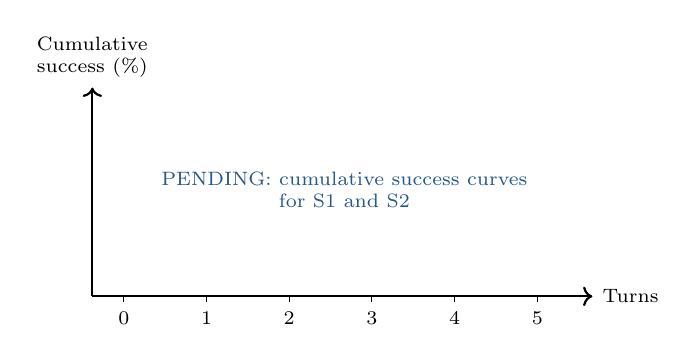
\begin{tikzpicture}[x=1cm,y=1cm,font=\scriptsize]
\draw[->,thick] (.7,.55)--(7.05,.55) node[right] {Turns};
\draw[->,thick] (.7,.55)--(.7,3.2) node[above,align=center] {Cumulative\\success (\%)};
\foreach \i/\x in {0/1.1,1/2.15,2/3.2,3/4.25,4/5.3,5/6.35}{\draw (\x,.55)--(\x,.48) node[below] {\i};}
\node[align=center,text=deepblue] at (3.9,1.9) {PENDING: cumulative success curves\\for S1 and S2};
\end{tikzpicture}
\caption{Temporary plotting template: eventual task success by clarification turn. No data plotted.}
\label{fig:clarification}
\end{figure}
\noindent\textbf{Results commentary to complete (placeholder).}  In the completed report, explain how often clarification is needed, how quickly it resolves missing information, and whether repeated review reduces unnecessary questions. Report the linked-dependency subgroup separately, with its sample count and uncertainty, rather than claiming a broad effect from a small subgroup.

\noindent\textit{Planned reporting detail.} The zero-turn point records tasks already correct before any question is asked. Later points count only cases that become correct after receiving the corresponding clarification answer. The completed analysis will separate cases that were unnecessarily queried from cases where clarification was necessary but unsuccessful.

\FloatBarrier
\section{Discussion}
\pending{Reserved for interpretation of verified findings, limitations, and comparison with prior work.}
\section{Conclusion and Future Work}
\pending{Reserved until results and discussion have been completed.}
\section*{Code and Data Availability}
The project repository is available at \url{https://github.com/huziibee/Research_Project}. Dataset release conditions, final evaluation splits, and reproducibility artifacts will be specified after the experimental protocol is frozen.
\section*{Acknowledgements}
All praise and thanks are due to Allah, whose mercy, guidance, and blessings made this work possible, and who granted me the strength, patience, and perseverance to complete it. I am deeply grateful to my supervisors, Steven James and Benjamin Rosman, for their guidance, feedback, encouragement, and for continually helping me strengthen the clarity and rigour of this research. I would also like to thank my parents, Mohammed Ebrahim Bangie and Gulshan Bangie, for their unwavering support, patience, encouragement, and sacrifices throughout my studies. Finally, I thank Taruna Naidoo for her support and helpful advice during the preparation of this research report.
\begin{thebibliography}{99}
\bibitem{ambik} A. Ivanova \emph{et al.}, ``AmbiK: Dataset of Ambiguous Tasks in Kitchen Environment.''
\bibitem{tool} Y. Zhang \emph{et al.}, ``Can You Pass That Tool?: Implications of Indirect Speech in Physical Human-Robot Collaboration.''
\bibitem{clara} J. Park \emph{et al.}, ``CLARA: Classifying and Disambiguating User Commands for Reliable Interactive Robotic Agents,'' \emph{IEEE Robotics and Automation Letters}, 2023.
\bibitem{clarifyvc} H. Zhou \emph{et al.}, ``ClarifyVC: Clarifying Ambiguous Commands in Vehicle Control with a Hybrid Data Augmentation Pipeline,'' \emph{ICLR}, 2026.
\bibitem{codraw} B. Madureira and D. Schlangen, ``Instruction Clarification Requests in Multimodal Collaborative Dialogue Games: Tasks, and an Analysis of the CoDraw Dataset.''
\bibitem{sarathy} V. Sarathy, M. Fawn, M. McWilliams, M. Scheutz, and B. Oosterveld, ``On Evaluating LLM Integration into Robotic Architectures.''
\bibitem{mannekote} A. Mannekote \emph{et al.}, ``Making Task-Oriented Dialogue Datasets More Natural by Synthetically Generating Indirect User Requests.''
\bibitem{searle1975} J. R. Searle, ``Indirect Speech Acts, in \emph{Syntax and Semantics}, vol. 3, \emph{Speech Acts}, P. Cole and J. L. Morgan, Eds. New York: Academic Press, 1975, pp. 59--82.
\bibitem{grice1975} H. P. Grice, ``Logic and Conversation, in \emph{Syntax and Semantics}, vol. 3, \emph{Speech Acts}, P. Cole and J. L. Morgan, Eds. New York: Academic Press, 1975, pp. 41--58.
\bibitem{glm52} GLM-5 Team, ``GLM-5: From Vibe Coding to Agentic Engineering, arXiv:2602.15763, 2026. GLM-5.2 model documentation: \url{https://huggingface.co/zai-org/GLM-5.2}.
\bibitem{grok45} SpaceXAI, ``Grok 4.5 Model Card, July 2026. \url{https://media.x.ai/v1/website/4p5-5184fdf9.pdf}.
\bibitem{gpt56sol} OpenAI, ``GPT-5.6 System Card, July 2026. Available: \url{https://deploymentsafety.openai.com/gpt-5-6}. GPT-5.6 Sol model documentation: \url{https://developers.openai.com/api/docs/models/gpt-5.6-sol}.
\bibitem{qwen} Qwen Team, ``Qwen3 Technical Report,'' 2025.
\bibitem{vague} H. Nam \emph{et al.}, ``VAGUE: Visual Contexts Clarify Ambiguous Expressions,'' \emph{Proc. ICCV}, 2025.
\end{thebibliography}
\end{document}
